%----------------------------------------------------------------------------
%----------------------------------------------------------------------------
%bb defines the bounding box for the pdf
%viewport defines the area of the pdf used
%in sidewaysfigure the last entry in bb moves the caption toward/away the pic
%in sidewaysfigure the second entry in bb moves the pic toward/away the caption
%----------------------------------------------------------------------------
\begin{figure}
\scalebox{0.8}[0.8]{
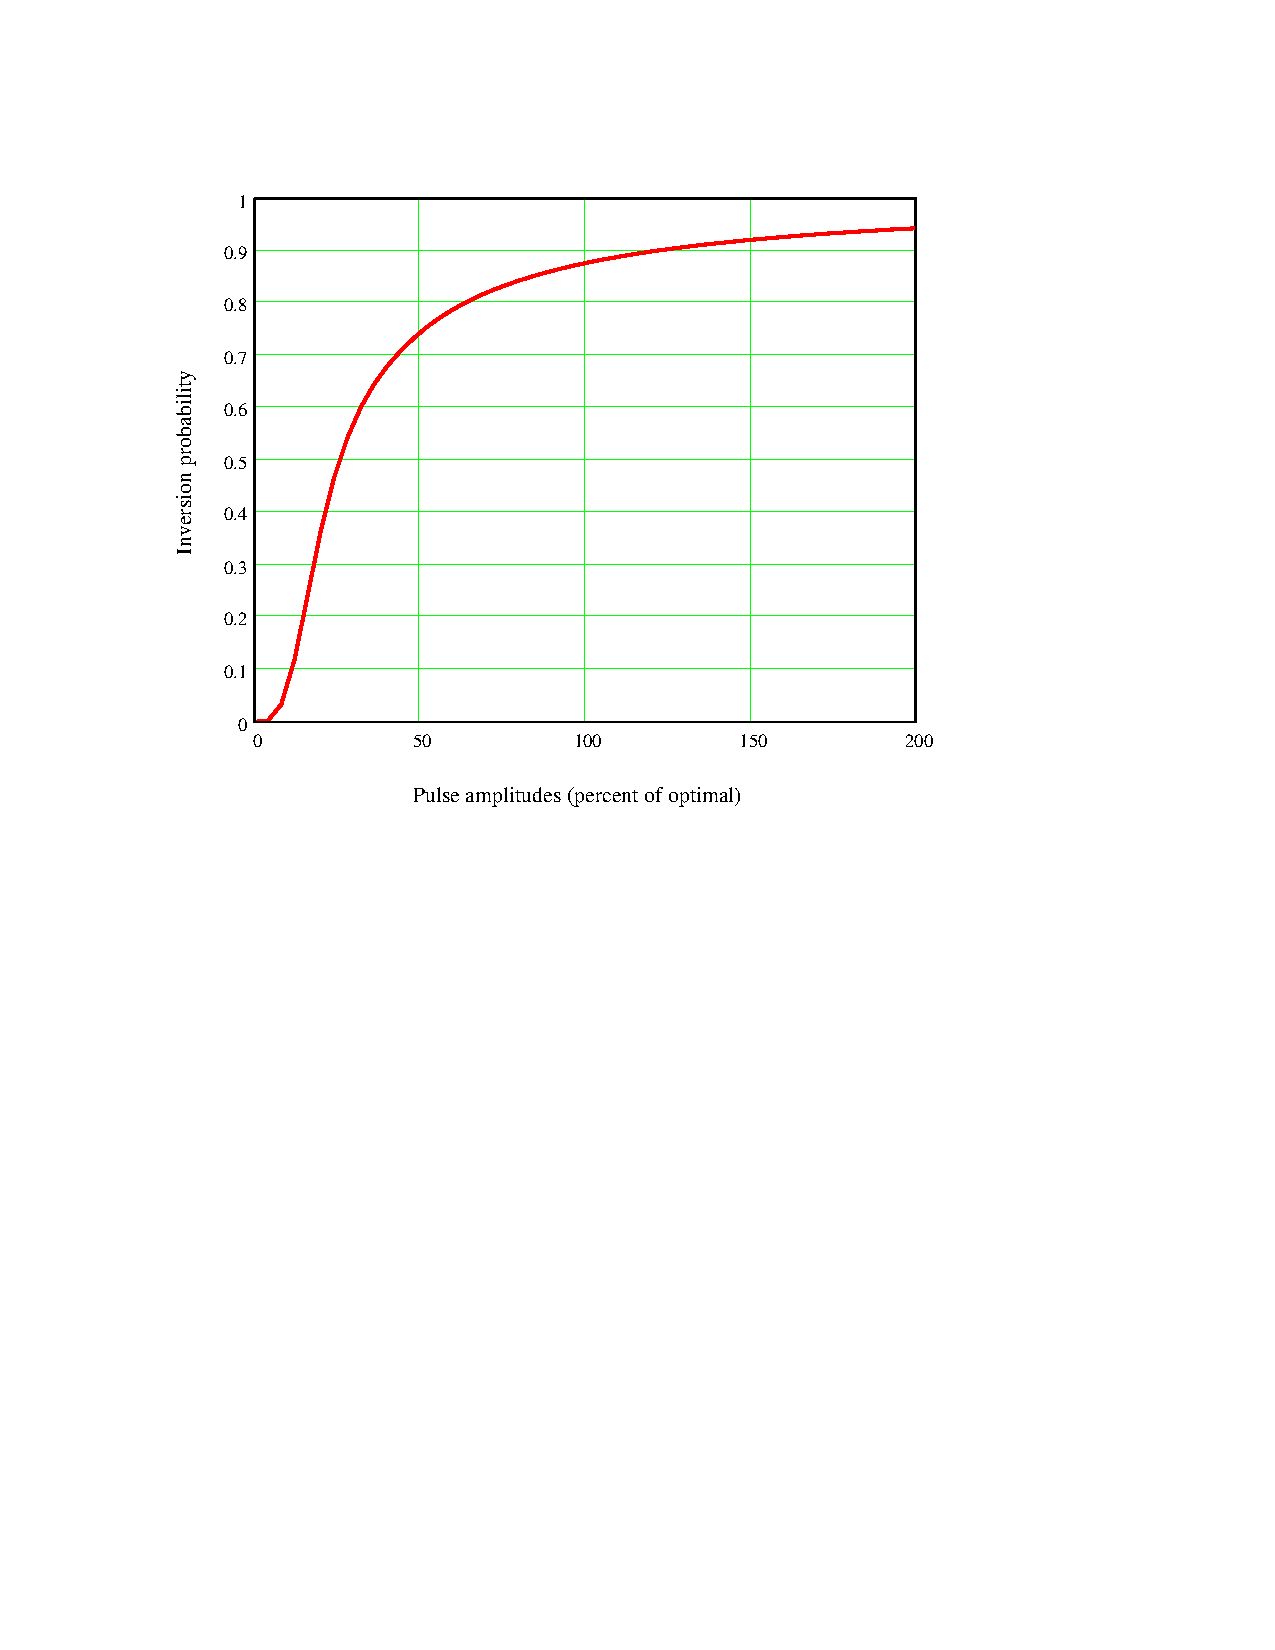
\includegraphics[bb=10 415 489 700]
{polarization/polarization.pdf}
}
\caption[STIRAP inversion of a randomly oriented ensemble]{STIRAP inversion of a randomly oriented ensemble. Compare this with the dynamics shown in Figure \ref{dynamics} and we see that the STIRAP process approaches a coherent 100\% inversion in the semi--classical analysis of a randomly orientated ensemble while the standard single color method of inverting the ensemble tends toward an incoherent 50\% inversion with oscillations.}
\label{polarization}
\end{figure}
%----------------------------------------------------------------------------

%----------------------------------------------------------------------------
The robust features of the STIRAP with respect to pulse heights has more advantages than the resistance to amplitude instabilities of the laser source (explored in Section \ref{random sims}). Here we examine its effect on the ``polarization damping'' studied in Section \ref{polarization damping}. The pulse amplitudes are allowed to vary as a pair (the pulses remain of equal height) and an average similar to Equation \ref{initial eom} is calculated using a numerical integration. In Figure \ref{polarization}, we see that even at ``only'' 100\% of the optimal pulse height over 85\% of the population is inverted and at 200\% of optimal the population inversion approaches 95\%
%----------------------------------------------------------------------------
%----------------------------------------------------------------------------
%----------------------------------------------------------------------------
